\documentclass[11pt]{article}

\usepackage[margin=1in]{geometry}
\usepackage[T1]{fontenc}
\usepackage[utf8]{inputenc}
\usepackage{lmodern}
\usepackage{microtype}
\usepackage{amsmath, amssymb, amsthm, mathtools}
\usepackage{bm}
\usepackage{enumitem}
\usepackage{graphicx}
\usepackage{hyperref}
\usepackage{xcolor}
\usepackage{xypic}
\usepackage[all,line,color]{xy}
\usepackage{graphicx}
\usepackage{pagecolor}
\pagecolor{white}
\usepackage{hyperref}
\usepackage{wrapfig
}\usepackage{caption}
\usepackage{tikz}
\usetikzlibrary{arrows.meta}
\usepackage{amsmath,amssymb}
\usepackage{algorithm}
\usepackage{algpseudocode}

% Define the custom inline macro
\DeclareRobustCommand{\externallink}{%
  \tikz[
    x=1ex,
    y=1ex,
    baseline=-0.05ex,
    line width=0.18ex,
    line cap=round,
    line join=round
  ]{%
    % outer box, intentionally open at top-right
    \draw (0,0) -- (0,1.05) -- (0.68,1.05);
    \draw (0,0) -- (1.05,0) -- (1.05,0.68);

    % arrow corner
    \draw (0.78,1.25) -- (1.25,1.25) -- (1.25,0.78);

    % arrow shaft
    \draw[-{Stealth[length=0.32ex,width=0.28ex]}]
      (0.48,0.48) -- (1.28,1.28);
  }%
}

\captionsetup[figure]{
  format=plain,
  justification=justified,
  singlelinecheck=false,
  margin=1.75cm,
  font=small
}

\hypersetup{
    colorlinks=true,
    linkcolor=blue!50!black,
    citecolor=blue!50!black,
    urlcolor=blue!50!black,
    pdftitle={Problem agnostic hierarchies, path-volume, and log speed-up in RL},
    pdfauthor={Tyler Foster}
}

\author{Tyler Foster}
\date{\today}

\newtheorem{definition}[subsubsection]{Definition}
\newtheorem{assumption}[subsubsection]{Assumption}
\newtheorem{assumptions}[subsubsection]{Assumptions}
\newtheorem{construction}[subsubsection]{Construction}
\newtheorem{example}[subsubsection]{Example}
\newtheorem{remark}[subsubsection]{Remark}
\newtheorem{ermark}[subsubsection]{}
\newtheorem{warning}[subsubsection]{Warning}
\newtheorem{question}[]{Question}
\newtheorem{theorem}[subsubsection]{Theorem}
\newtheorem{proposition}[subsubsection]{Proposition}
\newtheorem{lemma}[subsubsection]{Lemma}
\newtheorem{corollary}[subsubsection]{Corollary}
\newtheorem{principle}[subsubsection]{Principle}
\newtheorem{run_analysis}[subsubsection]{Runtime analysis}


\newcommand{\Act}{\mathsf{A}}
\newcommand{\src}{\operatorname{src}}
\newcommand{\tgt}{\operatorname{tgt}}
\newcommand{\Path}{\operatorname{Path}}
\newcommand{\Hist}{\operatorname{Hist}}
\newcommand{\supp}{\operatorname{supp}}
\newcommand{\Vol}{\operatorname{Vol}}
\newcommand{\E}{\mathbb{E}}
\newcommand{\R}{\mathbb{R}}
\newcommand{\N}{\mathbb{N}}
\newcommand{\PVol}{\mathcal{P}\text{-}\mathrm{Vol}}
\newcommand{\TV}{\operatorname{TVol}}
\newcommand{\diam}{\operatorname{diam}}
\newcommand{\im}{\operatorname{im}}
\newcommand{\id}{\operatorname{id}}
\newcommand{\cost}{\operatorname{Cost}}
\newcommand{\fiber}{\operatorname{Fib}}
\newcommand{\quot}{\mathbin{/}}
\newcommand{\localfigdir}{assets/images/mathematical_model}
\newcommand{\projectfigdir}{../../assets/images/mathematical_model}

% Prefer local bundled figures when this draft is compiled from the zip.
% If this file is dropped into docs/design/ inside the repository, fall back
% to the repository's existing assets directory. If neither exists, preserve
% the figure slot as an explicit placeholder rather than silently deleting it.
\newcommand{\safeincludegraphics}[2][]{%
  \IfFileExists{\localfigdir/#2}{%
    \includegraphics[#1]{\localfigdir/#2}%
  }{%
    \IfFileExists{\projectfigdir/#2}{%
      \includegraphics[#1]{\projectfigdir/#2}%
    }{%
      \fbox{\begin{minipage}[c][1.55in][c]{0.82\linewidth}
        \centering\small Figure file preserved but not found in this build:\\
        \texttt{#2}
      \end{minipage}}%
    }%
  }%
}

\begin{document}


The shared concrete mechanism is:

\[
\text{multiplicative scale}
\quad\longrightarrow\quad
\text{additive depth},
\]
\[
\text{fine metric detail}
\quad\longrightarrow\quad
\text{coarse order or valuation data},
\]
\[
\text{ordinary geometry}
\quad\longrightarrow\quad
\text{tree, fan, quotient skeleton}.
\]

For tropicalization with \(0<b<1\), the meaningful expression is not a fixed
\(\log_b(x)\) as \(b\to 0\), since fixed \(x\) mostly degenerates. The meaningful
move is to write

\[
x(b) = b^a,
\]

so that

\[
\log_b x(b) = a.
\]

\begin{figure}[!ht]
    \vskip -.5cm
    $$
    \!\!\!\!\!\!\!\!\!\!\!\!\!\!\!\!\!\!\!\!
    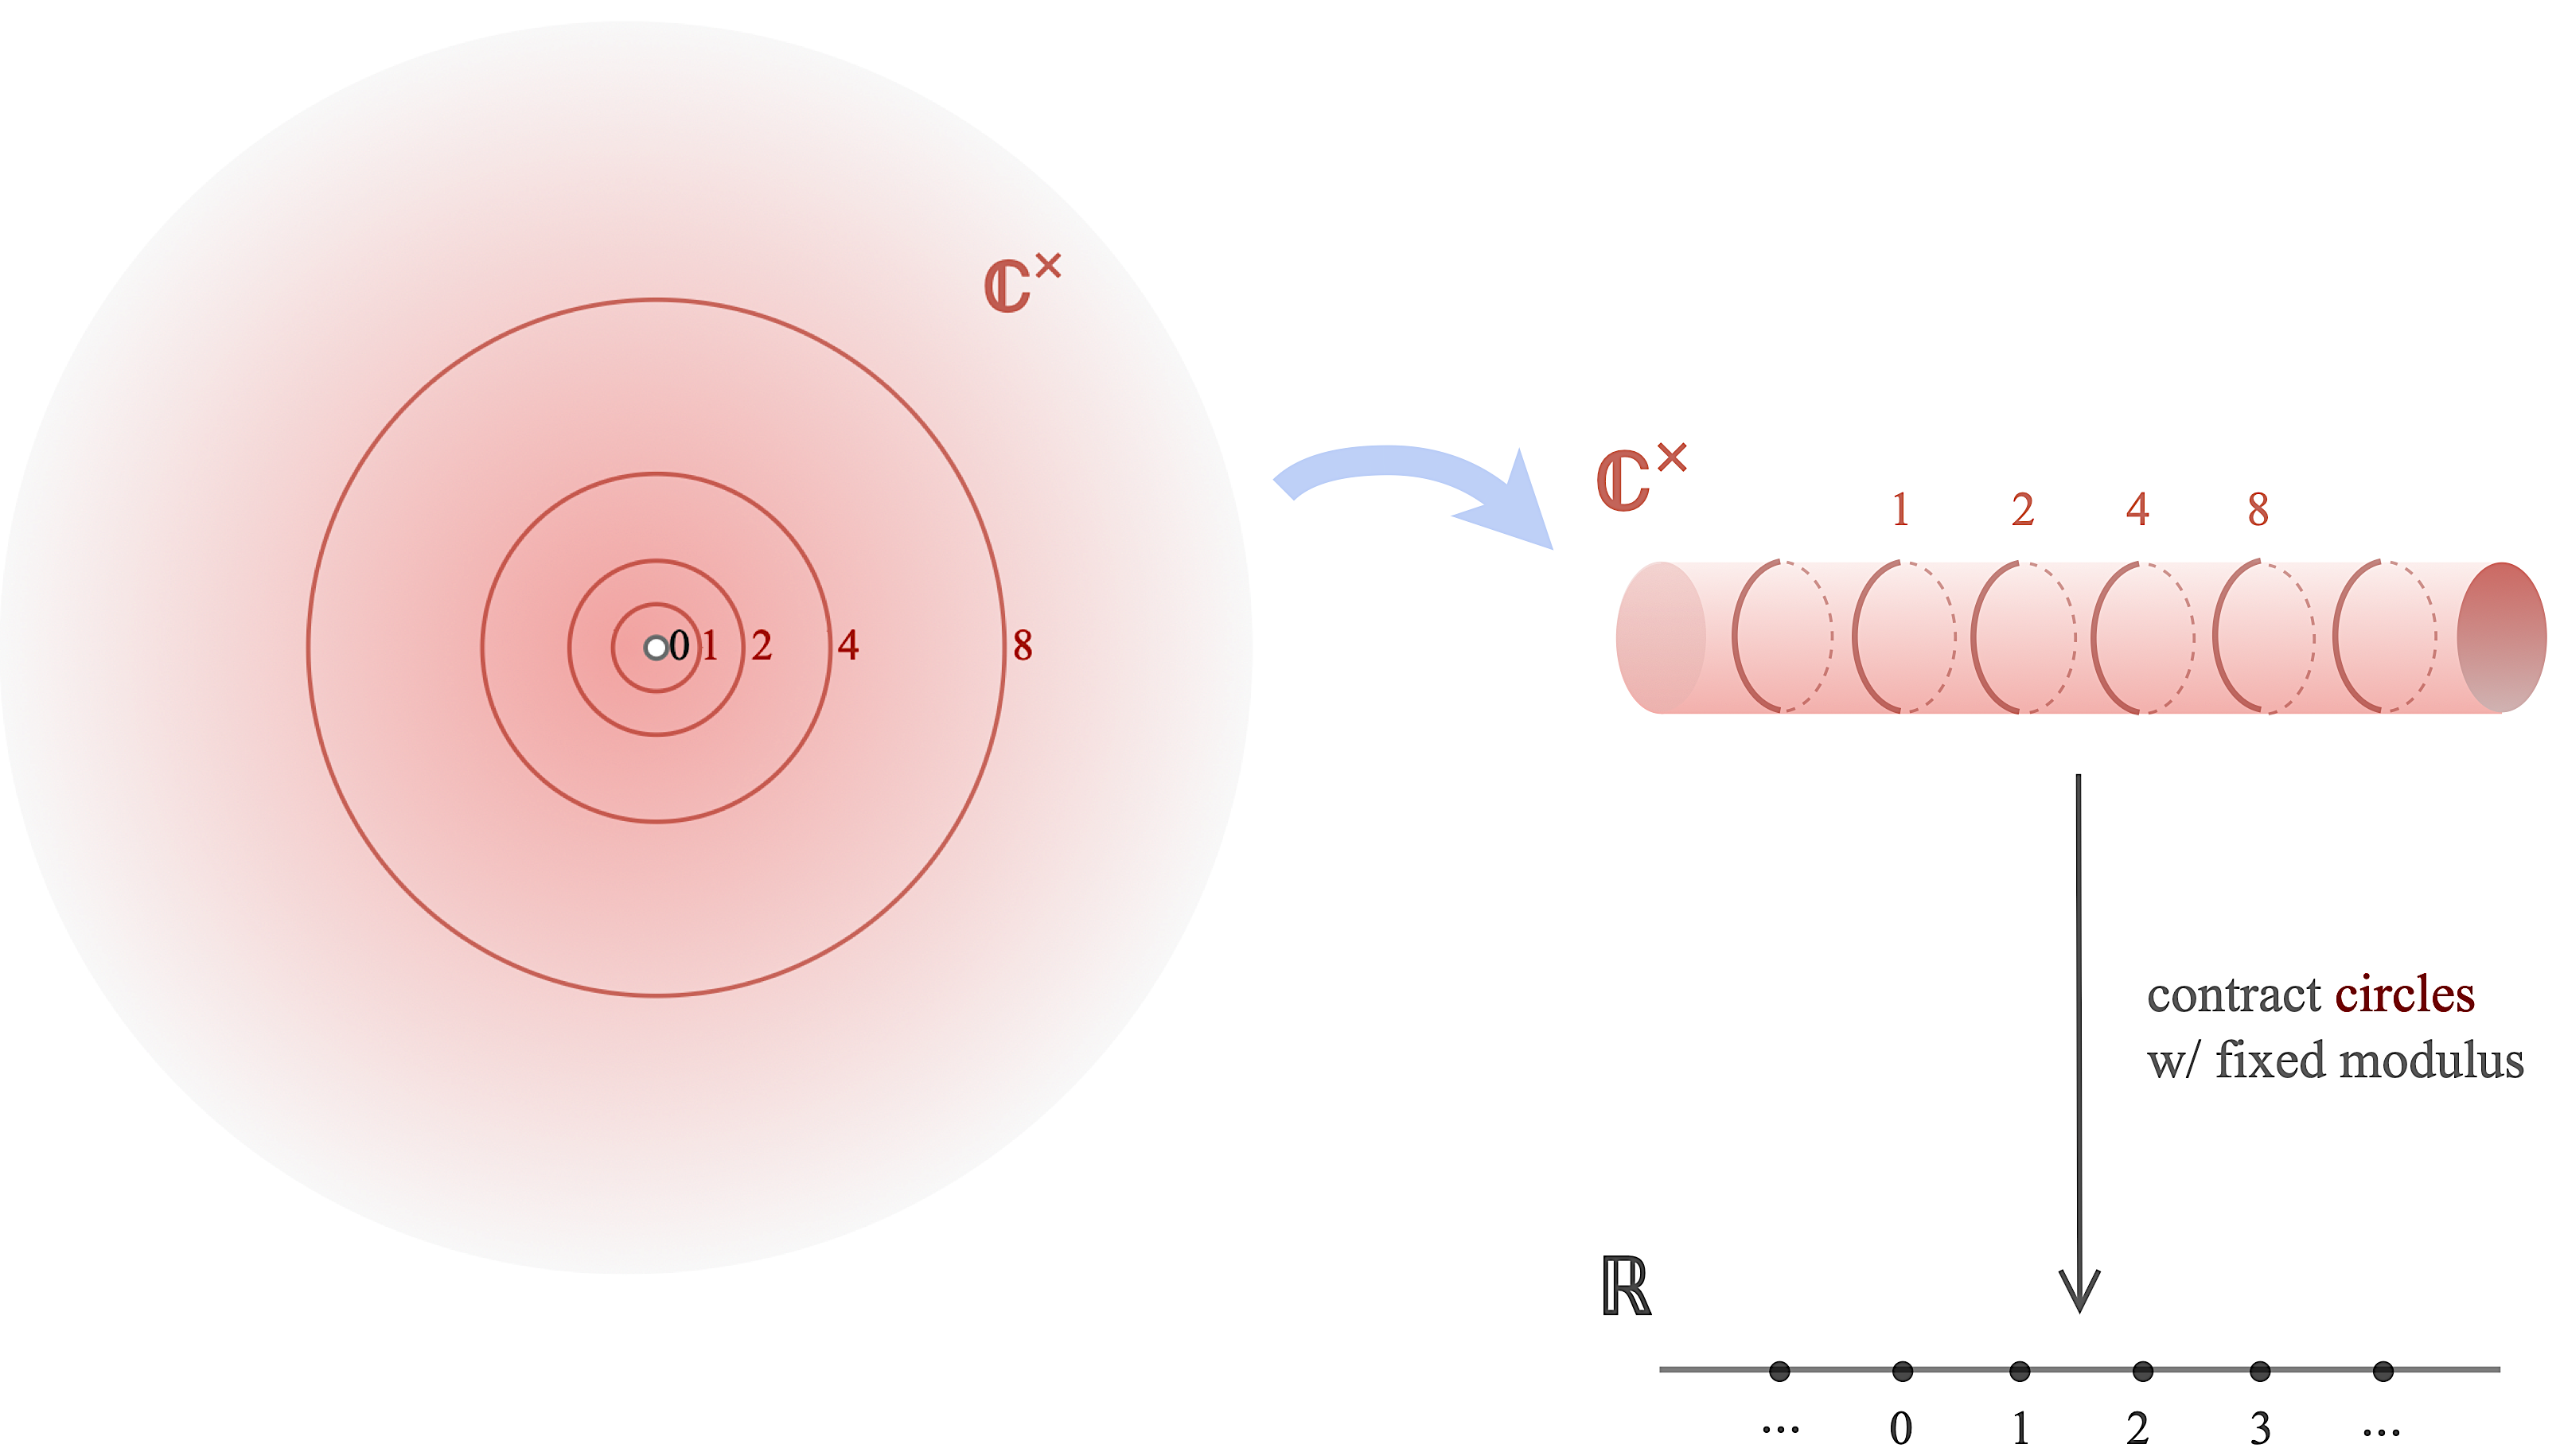
\includegraphics[scale=0.28]{assets/images/Ctimes.png}
    $$
    \vskip -.5cm
    \caption{[...]}
    \label{fig:Ctimes}
\end{figure}

For sums, one obtains

\[
\log_b\!\left(b^a + b^c\right) \longrightarrow \min(a,c)
\qquad \text{as } b\to 0.
\]

Thus tropicalization says:

\[
\text{keep the exponent or scale;}
\]
\[
\text{throw away coefficient-level detail;}
\]
\[
\text{turn addition into } \min;
\]
\[
\text{turn multiplication into addition.}
\]


\begin{figure}[!ht]
    \vskip -.5cm
    $$
    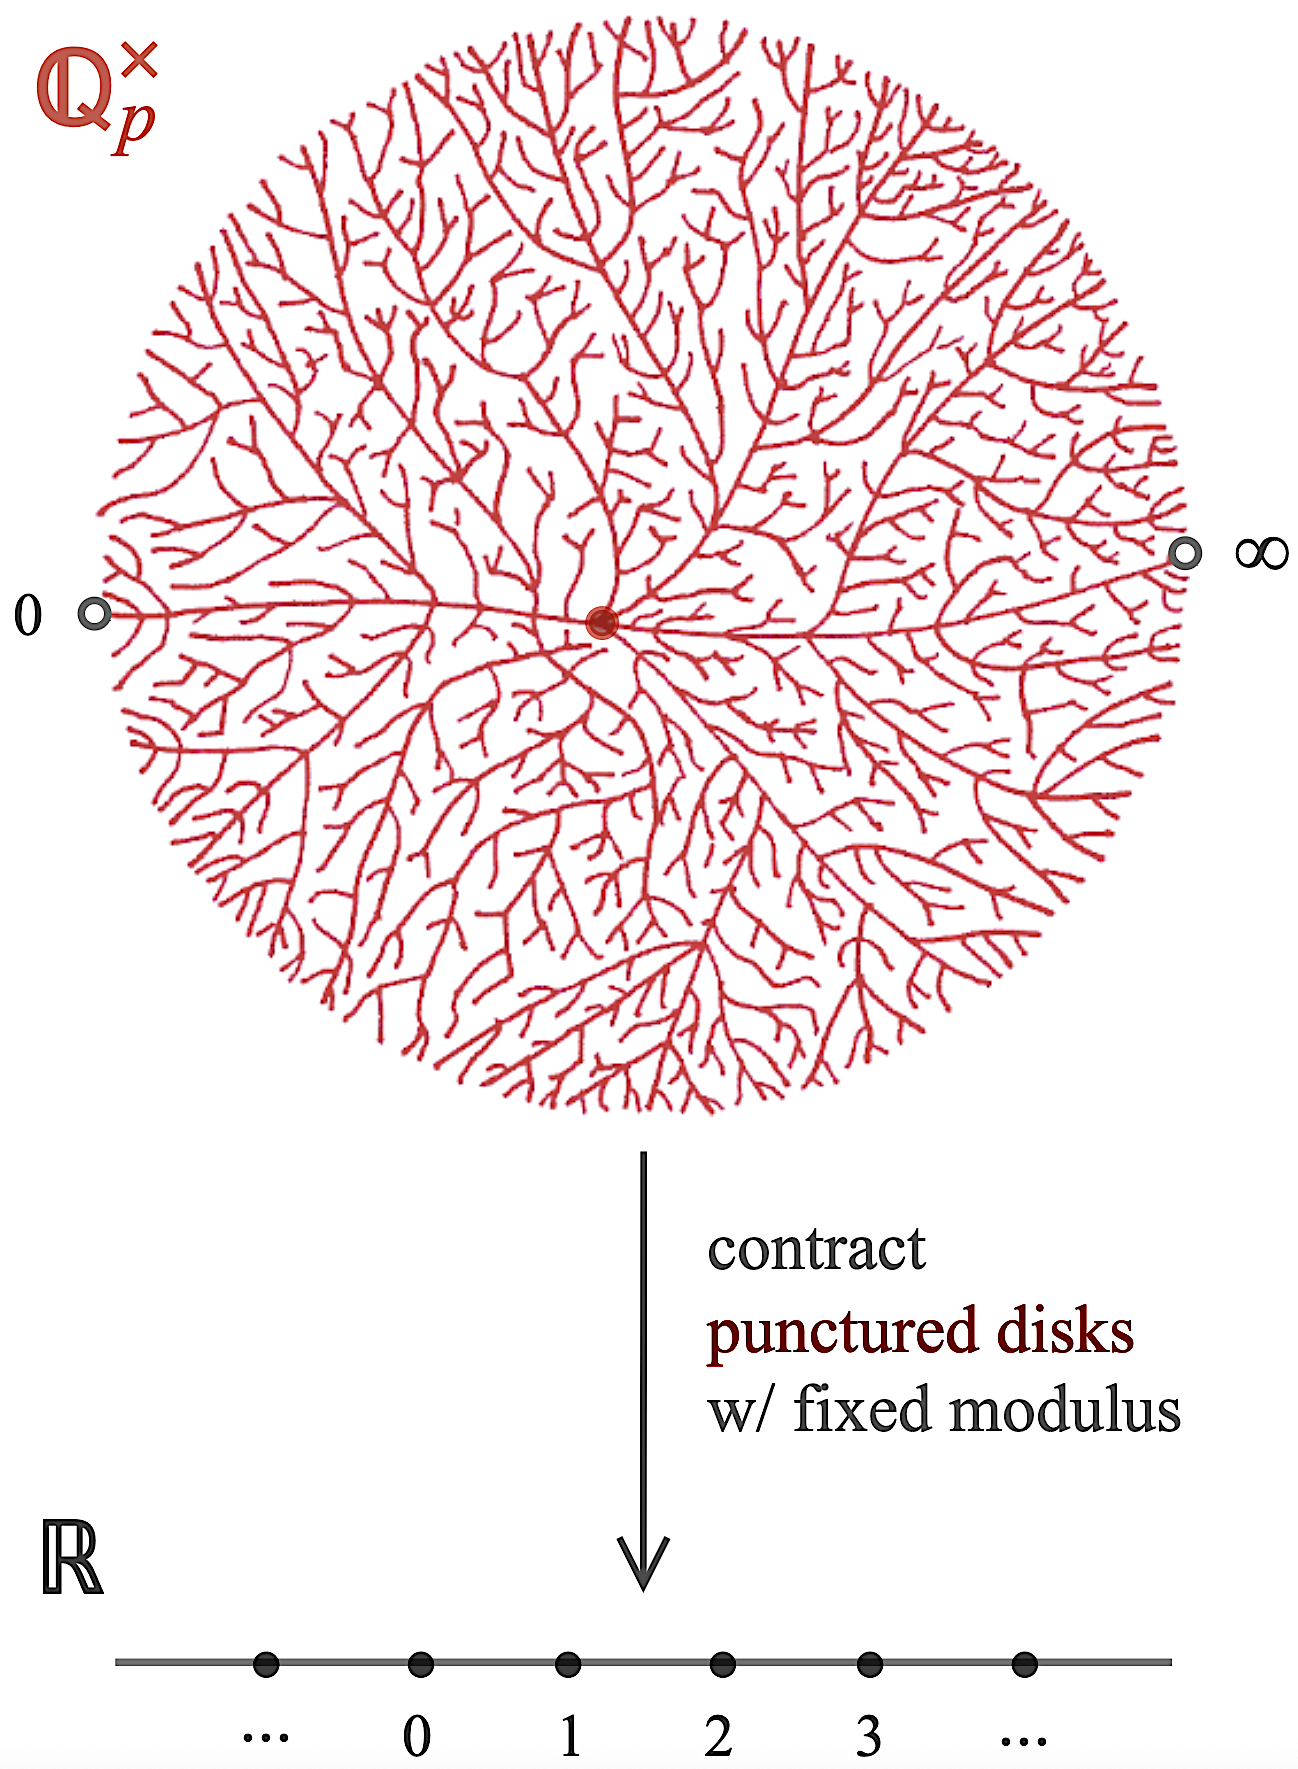
\includegraphics[scale=0.28]{assets/images/Qptimes.png}
    $$
    \vskip -.5cm
    \caption{[...]}
    \label{fig:Qptimes}
\end{figure}


Now compare the binary contraction tower. Take a dyadic grid. At depth \(k\),
cells have size

\[
2^{-k}.
\]

A binary quotient or coset tier forgets all detail below that scale. A point is
no longer ``this exact grid point''; it is ``this dyadic coset at depth \(k\).''
The important invariant becomes

\[
\text{scale} = 2^{-k},
\]

and therefore

\[
\text{depth} = -\log_2(\text{scale}) = k.
\]

So the binary tower is also doing:

\[
\text{keep the exponent or depth;}
\]
\[
\text{throw away within-cell detail.}
\]

That is the same move as tropicalization.

The deep reason these feel like the same phenomenon is that both are valuation
machines. A valuation converts size or order into an additive number:

\[
v(xy) = v(x) + v(y),
\]

and

\[
v(x+y) \geq \min(v(x),v(y)).
\]

In the tropical limit, this inequality becomes the governing rule:

\[
v(x+y) = \min(v(x),v(y))
\]

generically.

In the binary coset tower, the valuation is dyadic depth:

\[
v_2(\text{scale}) = \text{depth}.
\]

Equivalently, for two grid points,

\[
\text{distance scale} \sim 2^{-k}
\qquad\Longleftrightarrow\qquad
\text{separation depth} \sim k.
\]

Two points are indistinguishable until the tier where their binary addresses
split. The tower keeps that split-depth and discards the lower bits. That is a
tropical or ultrametric kind of geometry.

So a useful explanation is:

\begin{quote}
Tropicalization and binary contraction towers are both ways of replacing metric
magnitude by scale depth. The logarithm is not an extra analytic trick; it is
the coordinate change from multiplicative refinement to additive tier index.
\end{quote}

Or, more compactly:

\[
\text{tropicalization:}\qquad x=b^a \longmapsto a,
\]

\[
\text{binary tower:}\qquad \text{cell size}=2^{-k} \longmapsto k.
\]

Both say: the real object is not the tiny quantity itself, but the exponent at
which it lives.

That is why \(\lim_{b\to 0}\log_b\) and a tower of binary cosets can be
understood as manifestations of the same idea: each builds a limiting skeleton
where only dominance, scale, and ancestry survive.

\end{document}
